% Options for packages loaded elsewhere
%\PassOptionsToPackage{unicode}{hyperref}
%\PassOptionsToPackage{hyphens}{url}
%
\documentclass[11pt]{article}
\usepackage{amsmath,amssymb}
\usepackage{graphicx,psfrag,epsf}
\usepackage{enumerate}
\usepackage{lmodern}
\usepackage{rotating}
\usepackage[authoryear]{natbib}
\usepackage{authblk}
\usepackage{hyperref,float}
%\usepackage{cite}

\usepackage{hyperref}
\usepackage[margin=1in]{geometry}
\usepackage{iftex}
\ifPDFTeX
  \usepackage[T1]{fontenc}
  \usepackage[utf8]{inputenc}
  \usepackage{textcomp} % provide euro and other symbols
\else % if luatex or xetex
  \usepackage{unicode-math}
  \defaultfontfeatures{Scale=MatchLowercase}
  \defaultfontfeatures[\rmfamily]{Ligatures=TeX,Scale=1}
\fi
% Use upquote if available, for straight quotes in verbatim environments
\IfFileExists{upquote.sty}{\usepackage{upquote}}{}
\IfFileExists{microtype.sty}{% use microtype if available
  \usepackage[]{microtype}
  \UseMicrotypeSet[protrusion]{basicmath} % disable protrusion for tt fonts
}{}
\makeatletter

\@ifundefined{KOMAClassName}{% if non-KOMA class
  \IfFileExists{parskip.sty}{%
    \usepackage{parskip}
  }{% else
    \setlength{\parindent}{0pt}
    \setlength{\parskip}{6pt plus 2pt minus 1pt}}
}{% if KOMA class
  \KOMAoptions{parskip=half}}
\makeatother
\usepackage{xcolor}
\usepackage[margin=1in]{geometry}
\usepackage{longtable,booktabs,array}
\usepackage{calc} % for calculating minipage widths
% Correct order of tables after \paragraph or \subparagraph
\usepackage{etoolbox}
\usepackage{setspace}

%%%%%%%%%%%%%%%%%%%%%%%%%%%%%%%%%%%%%%%%%%%%%%%%%%%%%%%
%jbes
% NOTE: To produce blinded version, replace "0" with "1" below.
\newcommand{\blind}{0}


%%%%%%%%%%%%%%%%%%%%%%%%%%%%%%%%%%%%%%%%%%%%%%%%%%%%%%%%

\makeatletter
%\patchcmd\longtable{\par}{\if@noskipsec\mbox{}\fi\par}{}{}
\makeatother
% Allow footnotes in longtable head/foot
\IfFileExists{footnotehyper.sty}{\usepackage{footnotehyper}}{\usepackage{footnote}}
\makesavenoteenv{longtable}
\usepackage{graphicx}
\makeatletter
\def\maxwidth{\ifdim\Gin@nat@width>\linewidth\linewidth\else\Gin@nat@width\fi}
\def\maxheight{\ifdim\Gin@nat@height>\textheight\textheight\else\Gin@nat@height\fi}
\makeatother
% Scale images if necessary, so that they will not overflow the page
% margins by default, and it is still possible to overwrite the defaults
% using explicit options in \includegraphics[width, height, ...]{}
\setkeys{Gin}{width=\maxwidth,height=\maxheight,keepaspectratio}
% Set default figure placement to htbp
\makeatletter
\def\fps@figure{htbp}
\makeatother
\setlength{\emergencystretch}{3em} % prevent overfull lines
\providecommand{\tightlist}{%
  \setlength{\itemsep}{0pt}\setlength{\parskip}{0pt}}
\setcounter{secnumdepth}{5}
\newlength{\cslhangindent}
\setlength{\cslhangindent}{1.5em}
\newlength{\csllabelwidth}
\setlength{\csllabelwidth}{3em}
\newlength{\cslentryspacingunit} % times entry-spacing
\setlength{\cslentryspacingunit}{\parskip}
\newenvironment{CSLReferences}[2] % #1 hanging-ident, #2 entry spacing
 {% don't indent paragraphs
  \setlength{\parindent}{0pt}
  % turn on hanging indent if param 1 is 1
  \ifodd #1
  \let\oldpar\par
  \def\par{\hangindent=\cslhangindent\oldpar}
  \fi
  % set entry spacing
  \setlength{\parskip}{#2\cslentryspacingunit}
 }%
 {}
\usepackage{calc}
\newcommand{\CSLBlock}[1]{#1\hfill\break}
\newcommand{\CSLLeftMargin}[1]{\parbox[t]{\csllabelwidth}{#1}}
\newcommand{\CSLRightInline}[1]{\parbox[t]{\linewidth - \csllabelwidth}{#1}\break}
\newcommand{\CSLIndent}[1]{\hspace{\cslhangindent}#1}
\usepackage{tabularx}
\usepackage{longtable}
\usepackage{array}
\usepackage{colortbl}
\ifLuaTeX
  \usepackage{selnolig}  % disable illegal ligatures
\fi
\IfFileExists{bookmark.sty}{\usepackage{bookmark}}{\usepackage{hyperref}}
\IfFileExists{xurl.sty}{\usepackage{xurl}}{} % add URL line breaks if available
\urlstyle{same} % disable monospaced font for URLs
\hypersetup{
  pdftitle={Investor opinion formation and the distribution of stock returns},
  pdfauthor={Maria Osipenko, Rui Ren},
  hidelinks,
  pdfcreator={LaTeX via pandoc}}

\def\keywords{\vspace{.5em}
{\textit{Keywords}:\,\relax%
}}
\def\endkeywords{\par}

\def\JEL{\vspace{.5em}
{\textit{JEL codes}:\,\relax%
}}
\def\endkeywords{\par}



\begin{document}

\def\spacingset#1{\renewcommand{\baselinestretch}%
{#1}\small\normalsize} \spacingset{1}

%%%%%%%%%%%
\if0\blind
{
  \title{\bf Investor opinion formation and the distribution of stock returns}
  \author{Maria Osipenko\hspace{.2cm}\thanks{Corresponding author: \href{mailto:osipenko@hwr-berlin.de}{\nolinkurl{osipenko@hwr-berlin.de}}}\\
    Hochschule für Wirtschaft und Recht Berlin\\
    and \\
    Rui Ren \\
    Universität Augsburg}
  \maketitle
} \fi

\if1\blind
{
  \bigskip
  \bigskip
  \bigskip
  \begin{center}
    {\LARGE\bf Investor opinion formation and the distribution of stock returns}
\end{center}
  \medskip
} \fi

\bigskip
%%%%%%%%%%%

%\onehalfspacing
\begin{abstract}
We study how the distribution of stock returns is influenced by investor sentiment by applying expectile regression to abnormal returns. Distinguishing between the different aspects of investor opinion - investor perception, attention, and associated sentiment - we use firm- and time-specific proxies for each of these aspects. We consider purely financial indicators and scheduled and unscheduled events in an interplay with news sentiment. We find that the majority of the effects depend on the expectile level, which itself can be understood as the 'state of the world' or 'extremeness level' of abnormal returns. While not always significant for the mean regression, the proxies of the investment opinion show significant effects on the conditional distribution of abnormal returns beyond its mean. Our expectile regression approach allows us to naturally generalize previous studies of conditional mean regression to higher conditional moments and estimate the impact of investor opinion thereon. Significant impacts of positive and negative sentiment on the shape of the conditional return distribution are traced via expectile-based measures of dispersion and skewness. Moreover, using the relation of expectiles to expected shortfall, we consider the expected-shortfall-point of view and explore the significance of the effects on the conditional expected shortfall as well.
\end{abstract}

\begin{keywords}
abnormal returns, expectile, expectile regression, expected shortfall, news sentiment
\end{keywords}
\begin{JEL}
C13, C21, G12
\end{JEL}

\newpage
\spacingset{1.8} % DON'T change the spacing!

\hypertarget{introduction}{%
\section*{Introduction}\label{introduction}}
\addcontentsline{toc}{section}{Introduction}

%The effects of public information arrival and polarity or sentiment of its content on stock return movements and the question whether they make up good predictors of the later have captured attention of many researches. However the results are somewhat unaligned.%devous. %fragmented and debatable.
Establishing the link between investor sentiment associated with certain information flow channels and stock return movements has captured the attention of many researches. The results are still somewhat unaligned.

For instance, \cite{DAS2007} observe that the message volume (regarded as optimistic sentiment) is positively correlated with stock volatility and negatively correlated with stock returns. \cite{luss2009} show that text features from news articles predict the size of the movement but not the direction. \cite{HAGENAU2013} and \cite{NGUYEN2015} are able to significantly improve their return forecasts by using sentiment from news or social media. \cite{SHANG2014} confirms a significant effect only for negative sentiment.  \cite{KIM2014} find no evidence for predictive power of sentiment neither on returns nor on volatility. \cite{smales2016} again relates returns and volatility changes to news sentiment. Recently, \cite{AUDRINO2020} and \cite{FANG2021} report an improvement in volatility forecasts when sentiment from news and social media is accounted for.

%For instance, \cite{HAGENAU2013} and \cite{NGUYEN2015} are able to significantly improve their return forecasts by using sentiment from news or social media. \cite{SHANG2014} find a significant effect of sentiment only related to negative announcements.  \cite{Antweiler2004} claim that the number and the extent of text messages influences stock volatility but not returns.  \cite{DAS2007} observe that the message volume (regarded as optimistic sentiment) is positively correlated with stock volatility but negatively correlated with stock returns. \cite{KIM2014} find no evidence for predictive power of sentiment neither on returns nor on volatility or trading volume. Recently, \cite{AUDRINO2020} and \cite{FANG2021} again report an improvement in volatility forecasts on using sentiment from news and social media. \cite{CAMPBELL1992} incorporates an asymmetric news-about-dividends impact on return volatility in a GARCH-type model. Further focusing on this effect and using broad firm specific news arrivals as a proxy for information flow \cite{KALEV2004} report significant effects on intraday and daily level. The authors write "when public news is released, market activity intensifies as a result of belief revisions caused by the divergence of opinions among traders". \cite{Maheu2004} also find empirical evidence for an asymmetric effect of positive and negative news on volatility jumps. The authors infer the positiveness or negativeness using the earnings surprises without any textual analysis of news content. Thereby they assume, that a positive surprise indicates positive news and vice versa. \cite{Luss2012} use textual features from news articles and support vector machines to predict the magnitude of stock returns. \cite{fuess2020} build upon a sentiment-augmented factor model for excess return and a lexicon-based sentiment assessment. They report a significant improvement in model performance due to the incorporated text information.

Thereby, there is no clear alignment on how to measure investor sentiment. Various ways has been undergone in order to assess investor sentiment in its broad sense. Overall, the existing approaches to measuring investor sentiment can be divided into two categories. The first one uses financial proxies to measure sentiment, as exemplified  in \cite{de1990noise}, \cite{barberis1998model}, \cite{baker2007investor}. Candidate methods of measuring sentiment cinclude financial indicators such as book-to-market ratios, earnings surprises, sizes (\cite{FRIEND1988}, \cite{FAMA1992},  \cite{KOTHARI1997}, \cite{PONTIFF1998}, \cite{Maheu2004}), and event indicators such as news arrivals, earnings announcements, search inquiries. \cite{BERKMAN2009} also argue that varying degree in differences in opinion regarding some stocks may influence their price dynamics around earnings announcements. Among other proxies for the opinion gap, they use shares turnover in the time span around earnings announcements. The authors argument that stocks with high degree of opinion differences are overpriced and earn lower return on earnings announcement days due to opinion alignment.

The second approach is to infer investor sentiment directly from the relevant textual documents. \cite{Su2021} classifies the related approaches into dictionary-based and machine-learning-based. The first ones rely on word lists with positive and negative words, where the most famous dictionaries  are Harvard (HV) and Loughran \& McDonald (LM) word lists (e.g. \cite{LOUGHRAN2011}, \cite{JEGADEESH2013}). Machine-learning-based approaches use statistical models to map the word content to a relevant variable such as return (e.g., \cite{Antweiler2004}, \cite{FANG2021}).

In this paper, we use financial proxies and dictionary-based news sentiment obtained using the HV and LM word lists. To structure this broad assessment of investor sentiment into smaller chunks, we adopt the three investor opinion formation channels of \cite{Su2021}: investor perception (risk perception and individual beliefs), captured by financial variables, event-related investor attention, and investor sentiment in a narrow sense, quantified by positive or negative earnings surprises and disctionary-based polarity of news content.%, as in \cite{FRANKEL2022}.

On the model side, the limited attention hypothesis (\cite{corwin2008} and \cite{Loh2010}) and the opinion divergence hypothesis (\cite{BERKMAN2009} and \cite{chatterjee2012}) shed light on the ways these particular aspects of investor opinion influence asset pricing. \cite{fuess2020} introduce aggregated investor sentiment in their asset pricing model. They show that the inclusion of the lexicon-based sentiment as a risk factor yields a better model performance.

In this paper, we analyse the impact of the three opinion formation aspects on the distribution of abnormal daily returns. Thereby, we encapsulate {\it investor attention} using the indicators of days around earnings announcements and news arrivals.  The aggregated {\it investor perception} is captured by financial fundamentals such as book-to-market ratios, sizes, shares turnover around earnings announcements, and reported earnings per share. Earnings surprises and dictionary-based polarity assessment of firm-specific news content are used to proxy {\it investor sentiment} in its narrow sense. Our choice of the proxies is based on the empirical evidence found in the previous literature provided below.

Besides the different approaches on the sentiment side, there is no consensus on which parameters of the conditional return distribution are affected. Significant effects were shown for the conditional return expectation (e.g., in \cite{HAGENAU2013} and \cite{NGUYEN2015}) and for  the conditional variance (e.g., in \cite{AUDRINO2020} and \cite{FANG2021}). \cite{Cao2002} argue that not only the second but also the third moments of return distribution are effected by information arrival due to inert "sidelined" investors. \cite{ENGELBERG2018} go beyond and close up the tails of the return distribution by considering return anomalies. They find a sign-changing asymmetric effect on information days. Recently, \cite{HE2022} confirms significant asymmetric sentiment effects on low and high quantiles of the return distribution.

In this paper, we estimate the effects of investor sentiment {\it{on the whole distribution} } of abnormal returns by breaking it down to a fine grid of tail indices. That way we are neither constrained to a particular distributional assumption nor to certain conditional moments of the return distribution.

A natural choice of such tail indices are quantiles (\cite{Koenker1978}) of the return distribution, $q_{\alpha}(r_{i,t})$, for a range of $\alpha$-values in $(0,1)$ capable of representing the whole return distribution without explicit distributional assumptions. By means of quantile regression for a set of $\alpha\in(0,1)$, distributional effects of investor opinion can be estimated. \cite{NI2015}, \cite{Ma2018}, \cite{ALNASSERI2021}, and \cite{HE2022} use quantile regression to address the distributional effects of sentiment. The authors find different effects for different quantile levels and point out that, overall, extreme markets are largely driven by investor sentiment.

Instead of using $\alpha$-quantiles for representing the conditional return distribution, an alternative measure, $\tau$-expectiles, introduced in \cite{Newey1987}, can be employed. The $\tau$-expectile is the real number, such that the $\tau$-proportion of the expected distance to it lies below and the $(1-\tau)$-proportion lies above it. As quantiles generalize the concept of the median, expectiles generalize the concept of the mean. Therefore, the expectile regression for a range of $\tau$-values in $(0,1)$ naturally generalizes the mean regression and is capable of capturing the effects on the whole distribution of returns in our case. This fact makes our analysis comparable with the previous findings based on the mean regression for $\tau=0.5$ on one hand and capable of capturing distributional effects for $\tau\in (0,1)\setminus\{0.5\}$ on the other.

In summary, our expectile regression approach allows to study heterogeneous effects over the whole distribution of returns breaking it down to different expectile levels (similar to quantile regression). As opposed to quantile regression, it covers the mean regression as a special case of $\tau=0.5$ and facilitates simple and efficient estimation and inference on the obtained parameters (see \cite{waltrup2015} on the efficiency of expectles, \cite{Barry2018} for inference).

%Using coefficient standard errors robust to serial and cross-sectional correlation, we confirm significant positive effect of the day before earnings announcements and a significant negative effect of news and earnings arrivals *on lower tail of return distribution* even if the polarity of the news and earnings surpises are positive. Our explanation for the effects connects to a trading strategy "buy on rumor, sell news". That is, some investors tend to buy equities with low returns when they expect their growth (the 'rumor' part)  (when they are believed to be underpriced) and sell low return stocks to ride on the hype of positive news arrivals.

Based on our expectile regression results, we confirm significant asymmetric effects of information arrivals with positive and negative sentiment on the shape of the conditional return distribution using non-parametric expectile-based measures of dispertion and skewness. Another advantage of our expectile-based approach lies in the risk management perspective. The well-known connection of expectiles to expected shortfall (\cite{Taylor2008}) makes our investigation of the factors impacting the expectiles of the returns potentially useful for risk management insights. Using the estimated effects from our conditional expectile model, we obtain plug-in estimates for the respective effects on the conditional expected shortfall and evaluate their significance via bootstrap.

The contribution of our paper is threefold. First, by incorporating all three investor opinion channels in our model, we  conduct a more comprehensive analysis of the respective effects, which makes our approach stand out from the previous related studies. Second, we estimate the effects of investor sentiment on the whole distribution of asset returns, breaking it down to a fine grid of tail indices - expectiles - avoiding any distributional assumptions or model constrains to particular conditional moments. Third, based on the connection of expectiles and expected shortfall, we obtain the estimated effects of investor sentiment directly on the expected shortfall of returns, which is highly relevant for risk management and uncovered in the existing studies.

The rest of the paper is organized as follows. First, we introduce our data and the variables we use to proxy the investor opinion formation channels. Next, we describe our conditional expectile model and present our estimation results.  A close up analysis of the effects on the resulting shape of the conditional return distribution and expected shortfall follows. Finally, we conclude and point to possible further research direction.

\hypertarget{proxies-for-investor-opinion-channels}{%
\section{Proxies for investor opinion formation channels}\label{proxies-for-investor-opinion-channels}}

We use data for NASDAQ stocks in the period April 2015 - August 2019 obtained from Bloomberg.
Our dependent variable is the abnormal return of NASDAQ stocks in the mentioned period, computed as the stock-specific return on the day of news arrival minus the Center for Research in Security Prices (CRSP) value-weighted market return. The associated data on the size, the book-to-market (btm) ratios, the share turnover, and the associated sentiment features from news articles build up the set of explanatory variables.

The textual corpus in this paper contains news articles from NASDAQ News and Insights and is downloaded from the \href{https://blockchain-research-center.com/}{Blockchain Research Center}. We select the top 100 companies regarding news frequency in the final data set. The stock ticker list is provided in the Appendix. All news articles published on weekends, holidays or after 4 pm on weekdays are merged with news articles on the next trading day.
Table \ref{tab:table00} in the Appendix describes the textual corpus used to calculate dictionary-based investor sentiment measures.


We combine this data with the records on earnings announcement dates, information on earnings per share and on average earnings forecasts from the kaggle platform (accessed on
21.September 2022: 
https://www.kaggle.com/datasets/tsaustin/us-historical-stock-prices-with-earnings-data) and with the sector information from NASDAQ website https://www.nasdaq.com/market-activity/stocks/screener (accessed on 10 September 2022).

Based on the available data and on previous findings in the literature, we construct the proxies for the three channels of information flow: investor attention, investor sentiment and investor perception described in the following.

\vspace{0.5cm}
{\bf {Investor attention}}

\cite{chen2022},  \cite{daniel2020} and \cite{dellavigna2009}, among others, highlight the impact of investor attention on financial markets. \cite{dellavigna2009} refer to earnings announcements on different weekdays to capture the phenomena. \cite{daniel2020} focus on optimal attention allocation to news in investor utility terms and point out that the optimal attention to news increases in uncertainty in their model. \cite{drake2017} use search volume, analysts' forecast revisions, financial statements downloads and the number of news releases to quantify the amount of attention in the cross-sectional comovement sense. The authors argue, that because of limited attention, investors focus rather on categories of stocks (e.g., belonging to the same industry) than on individual tickers when it comes to choosing a stock to buy from a large cross-section of stocks. \cite{YUAN2015} investigates the role of market-wide "attention-grabbing" events in capturing investor attention across time. The author points out that the rise in attention level causes investors to make trade decisions.

In the spirit of the studies mentioned above, earnings announcements and news arrivals must be a valid indicator of investor attention allocation available on a daily and stock level.

In summary, as the proxies for investor attention to particular stocks , we employ:

\begin{itemize}
\tightlist
\item
  Indicator of firm-specific news arrival at \(t\) \(news_{i,t}\),
\item
  Number of day-sector specific news at \(t\) normalized on the number of firms in the sector, \(news\_sector_{i,t}\), and the overall number of news for the whole portfolio arrived at \(t\) \(news\_day_{i,t}\),
\item
  Indicator of earnings announcements days \(ean_{i,t}\), as well as
\item
  Indicators of days before and after earnings announcements, \(pre\_ean_{i,t}\) and \(post\_ean_{i,t}\).
\end{itemize}

The last two together indicate the time of news releases and a three-day period around the earnings announcements as in \cite{BERKMAN2009}.

\newpage
{\bf {Investor perception}}

We infer investor perception using variables which are relevant for risk assessment.
First, according to \cite{FRIEND1988}, the well-known size effect reflects risk levels and enters, therefore, our proxy for investor risk perception.
Second, \cite{Peasnell1982} connects the value of stocks and the expectation of future abnormal earnings by:

\[v_{i,t}= bv_{it} + \sum_{h=1}^\infty \frac1{(1+r)^h}\mathbb E_t(r_{i,t+h}^a)\]

where $v_{i,t}$ is the market value and $bv_{i,t}$ is the book value of  equity $i$, $r_{i,t}^a$ is the abnormal return at $t$ and $r$ is the cost of capital. The resulting book-to-market (btm) ratio is:
\[btm_{i,t} = \frac{bv_{it}}{v_{i,t}},\]
encompassing investor expectations. Here we adopt firm-specific btm ratios of the previous period, $btm_{i,t-1}$, as a proxy for firm performance expectations.  As a further proxy of future performance expectations, we employ firm-specific reported earnings per share, scaled to the interval $[-1,1]$.

Next, according to \cite{BERKMAN2009}, the share turnover around earnings announcements can be an indicator of opinion differences and consequently overpriced stocks, which leads to price correction upon information arrival, as the authors argue. Therefore, we also control for this effect by including an interaction term between share turnover and days-around-earnings-announcements indicator, $days\_ean_{i,t}$, in our model. The latter indicates the announcement date itself, the day before and the day after the earnings announcement as in \cite{BERKMAN2009}.

Finally \cite{DONNELLY2014} writes "The intuition is that the prices of growth stocks are much more sensitive to earnings expectations than those of value stocks." and "Accordingly, their prices are more sensitive than value stocks to any earnings surprise regardless of the sign." Therefore, we also include the interaction term between btm ratio $<1$ and post-earnings announcements  days, computed as $(btm_{i,t-1}<1)\cdot post\_ean_{i,t}$, to control for this effect.

In summary, as the proxies for investor perception, we use:

\begin{itemize}
\tightlist
\item
Logarithm of the size of company \(i\),  \(\log(size_{i,t})\),
\item
Book-to-market ratio of company \(i\) in  the previous period,   \(btm_{i,t-1}\),
%\item Reported earnings per share,
\item
  Shares turnover around earnings announcements, $turn_{i,t-1}$$\cdot days\_ean_{i,t}$, where  \(days\_ean_{i,t}\) denotes the indicator of a three-day period around an earnings announcement of company \(i\),
\item
  The interaction term between small btm ratios and post-earnings announcements days $(btm_{i,t-1}\leq 1)$$\cdot post\_ean_{i,t}$.
\end{itemize}

{\bf {Investor sentiment}}

Investor sentiment in its narrow sense, understood as positive or negative polarity  (e.g., in \cite{FRANKEL2022}), has been measured with several techniques in the associated literature.

%Investor sentiment influences stock prices, which is widely accepted in academia \cite{de1990noise}, \cite{TETLOCK2007}, \cite{LOUGHRAN2011} and \cite{FRANKEL2022}. Now, the question is no longer, as it was a few decades ago, whether investor sentiment affects stock prices, but rather how to measure investor sentiment and quantify its distributional effects.
%As previously mentioned, different approaches to measuring sentiment have been proposed.
On one hand, financial proxies were used to track investor sentiment (e.g., \cite{de1990noise}, \cite{barberis1998model}, \cite{baker2007investor}). In addition to already coverred measures under investor perception channel, we include earnings per share (as e.g., in \cite{henry2006}) and earnings surprises (as e.g., in \cite{Maheu2004}) to capture investor sentiment on eanings announcement days.
%For instance, earnings surprises were useful in \cite{Maheu2004} to proxy investor sentiment.

One the other hand, investor sentiment can be directly inferred from textual documents, where a dictionary-based and supervised machine learning sentiment techniques stand out (see e.g., \cite{JEGADEESH2013} for dictionary based methods and \cite{FANG2021} who successfully use machine learning methods (random forest) to infer textual sentiment). The results of \cite{FANG2021} and \cite{FRANKEL2022} on using non-linear sentiment models suggest a possibly non-linear effect of sentiment, which we capture in our per-expectile model. For that reason, we use a simpler dictionary-based method and calculate NASDAQ news sentiment as the sum of the positive words minus the sum of the negative words divided by the sum of both positive and negative words. This measure of sentiment is also called the net tone, and is widely adopted in applications. Following prior research, we apply two dictionaries to disclosure sentiment: the Loughran \& McDonald (LM) business-context dictionary and the Harvard (HV) psychosociological dictionary.

%Accordingly, we use four sentiment measures: direct assessment via earnings per share as well as earning surprises and indirect inferring of sentiment using LM and HV dictionary based on NASDAQ textual documents.
In summary, as the proxies for investor sentiment, we use:

\begin{itemize}
\tightlist
\item
  Earnings surprise \(surp_{i,t}\), computed as the difference of the average analysts' forecast and reported earnings per share,
\item
  Dictionary-based polarity assessments of firm-specific news content, computed using the LM word list, \(lm\_tone_{i,t}\),
\item
  Dictionary-based polarity assessments of firm-specific news content, computed using the HV word list, \(hv\_tone_{i,t}\).
\end{itemize}

We normalize the considerred sentiment measures to the interval \([-1,1]\).

Overall, the assignment of the proxies to an investor opinion channel is somewhat rudimentary, since they are interconnected and blurred. Our classification is thus not the only one possible and should just give a structure to the analysed effects.

Exploratory data analysis provided in the Appendix supports our hypothesis that the considered covariates impact the location, scale and shape of the conditional return distribution. To capture the effects on the conditional return distribution, we represent it through its conditional expectiles. A practical estimator of the respective effects on the return distribution can be obtained by expectile regression.

\hypertarget{expectile-regression-for-the-panel-data-of-nasdaq-returns}{%
\section{Expectile regression estimation for the panel of abnormal returns}\label{expectile-regression-for-the-panel-data-of-nasdaq-returns}}

As mentioned in the introduction, conditional expectile regression extends the associated conditional mean regression and allows to assess the respective effects on the whole distribution of asset returns, breaking it down to a fine grid of expectiles. That way, we are neither constrained to a particular distributional assumption nor to certain conditional moments of the return distribution. In this section, we review the general set up of the conditional mean model for the panel data of abnormal returns and its generalization to the conditional expectile regression (ER).

\hypertarget{general-model-definition}{%
\subsection{General model definition}\label{general-model-definition}}

Consider the conditional mean model for the panel data of abnormal returns of firm \(i\) at time \(t\), denoted as (\(r_{i,t}\)), with \(i=1,\ldots,n\) and \(t=1,\ldots, T\):
\[r_{i,t} = \beta_0 + x_{i,t}^\top\beta + z_{i}^\top\gamma + u_{i} + \varepsilon_{i,t}.\]

Response \(r_{i,t}\) is the abnormal return of stock \(i\) at time \(t\), computed as specified in Section ``Data''. \(x_{i,t}\) is a vector of \(p\) time-varying predictors, and \(z_i\) is a vector of \(m\) time-invariant covariates for stock \(i\) at time \(t\) where the individual samples $\{\{x_{i,t}\}_{t=1}^T,z_i,\{r_{i,t}\}_{t=1}^T\}_{i=1}^n$ are independent. $u_i$s are the unobserved firm-specific random effects with finite second moments and $\mathbb E(u_i|x_{i,t},z_i)=0$ for all $i$ and $t$, and $\varepsilon_{i,t}$ are idiosyncratic error terms with finite second moments and $\mathbb E(\varepsilon_{i,t}|x_{i,t},z_i,u_i)=0$  for all $i$ and $t$.

The model can be rewritten as:

\[r_{i,t} = \beta_0 + x_{i,t}^\top\beta + z_{i}^\top\gamma+v_{i,t},\]

where \(v_{i,t} = u_{i} + \varepsilon_{it}\).

The conditional expectile regression of \cite{Newey1987} aims at finding the conditional expectile (given the covariates \(x_{i,t}\) and \(z_i\)):

\[e_{\tau,t}(r_{i,t})\equiv e_\tau(r_{i,t}|x_{i,t},z_i) = x_{i,t}^\top \beta_\tau + z_{i}^\top \gamma_\tau, i=1,\ldots, n, t=1,\ldots T,\]

or in terms of the responses \(r_{i,t}\):

\[r_{i,t} = x_{i,t}^\top \beta_\tau + z_{i}^\top \gamma_\tau + v_{\tau,i,t},\]

where \(v_{\tau,i,t}\) is the error term with \(e_\tau(v_{\tau,i,t}|x_{i,t},z_i)=0\) and \(\tau\in (0,1)\) is the expectile level which specifies the desired ``extremeness'' level as \cite{Kneib2013}.

The related estimator minimizes the expectile loss function:

\[\arg\min_{\beta\in\mathbb R^p\gamma\in\mathbb R^m}\frac 1n\sum_{i=1}^n\sum_{t=1}^T\rho_\tau\Big(r_{i,t} - x_{i,t}\beta - z_i\gamma\Big),\]

where \(\rho_\tau(y)=|\tau - \mathbf 1(y<0)|y^2\) is the expectile check function.

The resulting estimator has the form:
\[\hat\theta_\tau =\begin{pmatrix}\hat\beta_\tau\\ \hat\gamma_\tau\end{pmatrix} = \Big(\sum_{i=1}^n\sum_{t=1}^T\hat w_{i,t} (\tau)\tilde x_{i,t}\tilde x_{i,t}^\top\Big)^{-1}\Big(\sum_{i=1}^n\sum_{t=1}^T\hat w_{i,t} (\tau)\tilde x_{i,t}r_{i,t}\Big),\]

where $\tilde x_{i,t} = \begin{pmatrix} x_{i,t}\\z_i\end{pmatrix}$ and \(\hat w_{i,t}(\tau) = |\tau - \mathbf 1(r_{i,t}\leq x_{i,t}\hat\beta_\tau + z_i\hat\gamma_\tau)|\).

The value of $\hat\theta_\tau$ can be computed via iterative weighted asymmetric least squares as proposed by \cite{Newey1987} on pooled data. \cite{BARRY2016} show consistency and asymptotic normality of the pooled estimator under mild assumptions.
%That is,
%\[\sqrt{n}(\hat \theta_\tau - \theta_\tau)\rightarrow \mathcal N(0,H^{-1}\Sigma H^{-1})\]
%
%The variances-covariances matrix of the estimator can be estimated via:
%
%\[\hat H=X^\top\hat W X/n, \text{where } \hat W = diag(\hat w_{1,1}(\tau),\ldots,\hat w_{n,T})\]
%
%and \[\hat \Sigma = X^\top\hat W\hat v_{\tau,i,t}\hat v_{\tau,i,t}^\top\hat WX/n\]
%
%with $X=(X_1,\ldots, X_n)^\top$ and $X_i=(\tilde x_{i,1}^\top,\ldots,\tilde x_{i,T}^\top)^\top$.
The variances-covariances matrix of the estimator consistently estimated with the cluster- and serial correlation-robust covariance estimator. We compute robust standard error estimates for the ER-coefficients using R-Package sandwich (\cite{Zeileis2020}) allowing for heteroscedastic random effects and seriall correlation of the error terms.

\hypertarget{er-with-proxies-of-investor-opinion}{%
\subsection{Expectile regression with proxies of investor opinion}\label{er-with-proxies-of-investor-opinion}}

We utilize the conditional linear expectile model defined above for estimating the effects of investor opinion channels on individual conditional expectiles of abnormal returns \(e_{\tau,t}(r_{i,t})\). Our model specification is as follows:
\vspace{-0.5cm}
\begin{align}
e_{\tau,t}(r_{i,t}) = &\beta_{0,\tau}+\beta_{1,\tau}\cdot pre\_ean_{i,t} + \beta_{2,\tau}\cdot ean_{i,t} + \beta_{3,\tau}\cdot post\_ean + \beta_{4,\tau}\cdot news_{i,t} \nonumber\\
&+\beta_{5,\tau}\cdot news\_sector_{i,t} + \beta_{6,\tau}\cdot news\_day_{i,t}  + \beta_{7,\tau}\cdot \log(size_{i,t}) + \beta_{8,\tau} \cdot btm_{i,t-1} \nonumber\\
&+ \beta_{9,\tau}\cdot days\_ean_{i,t}\cdot turn_{i,t-1}+ \beta_{10,\tau}\cdot (btm_{i,t-1}<1)\cdot ean_{i,t} +  \beta_{11,\tau}\cdot surp_{i,t}\nonumber\\
& + \beta_{12,\tau}\cdot lm\_tone_{i,t} + \beta_{13,\tau}\cdot hv\_tone_{i,t} + \gamma_{1,\tau}^{\top}\cdot sector_{i}+ \gamma_{2,\tau}^\top\cdot firm_{i},\label{eq:mod0}
\end{align}

where time varying predictors $x_{i,t}$ include the proxies of investor opinion channels discussed in Section 1, and time-invariant regressors $z_i$ include the associated sector and firm dummy variables of the form \((0,0,\ldots,0,1,0,\ldots,0)\), denoted as \(sector_{i}\) and \(firm_{i}\), respectively.


%where the time varying predictors $x_{i,t}$ include:
%
%\begin{itemize}
%\item
%  \(r_{i,t}\): the abnormal return of stock \(i\) at time \(t\),
%\item
%  \(pre\_ean_{i,t}\): the indicator of the day before an earnings announcement of company \(i\) at \(t\),
%\item
%  \(ean_{i,t}\): the indicator of an earnings announcement of company \(i\) at \(t\),
%\item
%  \(post\_ean_{i,t}\): the indicator of the day after an earnings announcement of company \(i\) at \(t\),
%\item
%  \(news_{i,t}\): the indicator of a news report referred to company \(i\) at \(t\),
%\item
%  \(news\_sector_{i,t}\): the number of news reports for the sector of company \(i\) at \(t\) normalized to the sector size,
%\item
%  \(news\_day_{i,t}\): the number of news reports  for all considered companies at \(t\) normalized to portfolio size,
%\item
%  \(\log(size_{i,t})\): the logarithm of the size of the company,
%\item
%  \(btm_{i,t-1}\): the book-to-market ratio of company \(i\) in \(t-1\),
%\item
%  \(turn_{i,t-1}\): the share turnover of company \(i\) in \(t-1\),
%\item
%  \(days\_ean_{i,t}\): the indicator of a three-day period around an earnings announcement of company \(i\) at \(t\),
%%\item
% % \(eps_{i,t}\): the reported earnings per share of company \(i\) in \(t\),
%\item
%  \(surp_{i,t}\): the earnings surprise at \(t\) computed as the difference between earnings per share and the average analysts' forecast for company \(i\) at \(t\) scaled to the interval $[-1,1]$,
%\item
%  \(lm\_tone_{i,t}\) and \(hv\_tone_{i,t}\):  the news sentiment measures of company \(i\) at \(t\) obtained by using the LM and HV dictionaries, respectively. These measures are computed as \(\frac{\#\text{ of positive words} - \# \text{ of negative words}}{\#\text{ of positive words}+\# \text{ of negative words}}\) using the corresponding dictionary and are scaled to the interval $[-1,1]$.
%\end{itemize}
%
% Time-invariant regressors $z_i$ include the associated sector and firm dummy variables of the form \((0,0,\ldots,0,1,0,\ldots,0)\), denoted as \(sector_{i}\) and \(firm_{i}\), respectively.



\begin{small}
\begin{sidewaystable}

\caption{\label{tab:table1}Coefficients and $R^2$ of the ERRE models with investor opinion proxies and different $\tau$s.
                           The effects of investor attention, investor perception and investor sentiment
                           are highlighted in blue, green and orange respectively.}
\centering
\begin{tabular}[t]{l|l|l|l|l|l|l|l}
\hline
  & $\hat\beta_{0.01}$ & $\hat\beta_{0.05}$ & $\hat\beta_{0.1}$ & $\hat\beta_{0.2}$ & $\hat\beta_{0.3}$ & $\hat\beta_{0.4}$ & $\hat\beta_{0.5}$\\
\hline
Constant & -0.19126*** & -0.09005*** & -0.05874*** & -0.02884* & -0.01123 & 0.00285 & 0.01624\\
\hline
$pre\_ean_{i,t}$ & 0.01545*** & 0.00943*** & 0.00708*** & 0.00476*** & 0.0034*** & 0.00226*** & 0.00123\\
\hline
$ean_{i,t}$ & -0.03214*** & -0.01863*** & -0.01283*** & -0.00706*** & -0.0037*** & -0.00132 & 0.00069\\
\hline
$post\_ean_{i,t}$ & -0.01185 & -0.00422 & -0.00039 & 0.00255 & 0.00385 & 0.0046 & 0.00538\\
\hline
$news_{i,t}$& -0.01316*** & -0.00683*** & -0.00478*** & -0.00288*** & -0.00188*** & -0.00114*** & -0.0005*\\
\hline
$news\_sector_{i,t}$& 0.00113 & 0.00136 & 0.00138 & 0.00124* & 0.00116* & 0.00113* & 0.0011*\\
\hline
$news\_day_{i,t}$ & -0.01036* & -0.00826*** & -0.0067*** & -0.00472*** & -0.00335*** & -0.00226*** & -0.00132*\\
\hline
$\log(size_{i,t})$ & 0.00578* & 0.00244* & 0.0015* & 0.00062 & 0.0001 & -0.00032 & -0.00073*\\
\hline
$btm_{i,t-1}$  & -0.00034 & -0.00166 & -0.00115 & -0.00027 & 0.00049 & 0.00116 & 0.00177*\\
\hline
$turn_{i,t-1}$$\cdot days\_ean_{i,t}$ & -0.00985*** & -0.00566*** & -0.00401*** & -0.00249*** & -0.00168*** & -0.00104* & -0.00049\\
\hline
$(btm_{i,t-1}\leq 1)$$\cdot post\_ean_{i,t}$& -0.03952* & -0.02861*** & -0.02311*** & -0.01656*** & -0.01212*** & -0.0086* & -0.00568\\
\hline
$supr_{i,t}$ & 0.08266*** & 0.07232*** & 0.06672*** & 0.06209*** & 0.05882*** & 0.05752*** & 0.05764***\\
\hline
$lm\_tone_{i,t}$ & 0.00597*** & 0.00258*** & 0.00187*** & 0.00149*** & 0.00139*** & 0.00137*** & 0.00139***\\
\hline
$hv\_tone_{i,t}$  & 0.01456*** & 0.00822*** & 0.00608*** & 0.00407*** & 0.00303*** & 0.00228*** & 0.00165***\\
\hline
$R^2$ & 0.34518 & 0.20291 & 0.12951 & 0.06151 & 0.02741 & 0.00994 & 0.00425\\
\hline
\end{tabular}
\\
\centering
\begin{tabular}[t]{l|l|l|l|l|l|l|l}
\hline
  & $\hat\beta_{0.5}$ & $\hat\beta_{0.6}$ & $\hat\beta_{0.7}$ & $\hat\beta_{0.8}$ & $\hat\beta_{0.9}$ & $\hat\beta_{0.95}$ & $\hat\beta_{0.99}$\\
\hline
Constant & 0.01624 & 0.03065*** & 0.04858*** & 0.07415*** & 0.11919*** & 0.17252*** & 0.36491***\\
\hline
$pre\_ean_{i,t}$ & 0.00123 & 0.0002 & -0.00093 & -0.00235* & -0.00461*** & -0.00636*** & -0.00974***\\
\hline
$ean_{i,t}$ & 0.00069 & 0.00265* & 0.00491*** & 0.00801*** & 0.01322*** & 0.01944*** & 0.03681***\\
\hline
$post\_ean_{i,t}$ & 0.00538 & 0.0064* & 0.00802* & 0.01076* & 0.01611* & 0.02227* & 0.03184***\\
\hline
$news_{i,t}$ & -0.0005* & 0.00014 & 0.00084* & 0.00176*** & 0.00333*** & 0.00499*** & 0.00961***\\
\hline
$news\_sector_{i,t}$ & 0.0011* & 0.0011* & 0.00111* & 0.00115* & 0.00133 & 0.00165 & 0.00022\\
\hline
$news\_day_{i,t}$ & -0.00132* & -0.00047 & 0.00034 & 0.00119 & 0.00188 & 0.00192 & 0.00208\\
\hline
$\log(size_{i,t})$& -0.00073* & -0.00118*** & -0.00175*** & -0.0026*** & -0.0041*** & -0.00594*** & -0.01288***\\
\hline
$btm_{i,t-1}$ & 0.00177* & 0.00239*** & 0.00307*** & 0.00393*** & 0.00544*** & 0.00685*** & 0.00735*\\
\hline
$turn_{i,t-1}$$\cdot days\_ean_{i,t}$ & -0.00049 & 0.00005 & 0.00065 & 0.00144*** & 0.00289*** & 0.00412*** & 0.00692***\\
\hline
$(btm_{i,t-1}\leq 1)$$\cdot post\_ean_{i,t}$ & -0.00568 & -0.00304 & -0.00044 & 0.00243 & 0.00634 & 0.01039 & 0.02283*\\
\hline
$supr_{i,t}$ & 0.05764*** & 0.05878*** & 0.06115*** & 0.06526*** & 0.07182*** & 0.07787*** & 0.08042*\\
\hline
$lm\_tone_{i,t}$ & 0.00139*** & 0.00145*** & 0.00155*** & 0.00173*** & 0.00201*** & 0.0022*** & 0.00115\\
\hline
$hv\_tone_{i,t}$ & 0.00165*** & 0.00108* & 0.00048 & -0.00019 & -0.00124 & -0.00196 & -0.00293\\
\hline
$R^2$ & 0.00425 & 0.00903 & 0.02559 & 0.05983 & 0.13159 & 0.20911 & 0.37607\\
\hline
\end{tabular}
\end{sidewaystable}
\end{small}

Within our model, we control for the effects of investor attention (\(\beta_1\) to \(\beta_6\)), the effects of investor perception (\(\beta_7\) to \(\beta_{10}\)), as well as the effects of investor sentiment (\(\beta_{11}\) to \(\beta_{13}\)).

We fit the models as specified in Equation \eqref{eq:mod0} for \(\tau\in\{0.05,0.1,\ldots,0.95\}\) and show the resulting coefficients, their significance (based on robust standard errors) and the associated \(R^2\) in Table \ref{tab:table1}.

\begin{figure}[h!]
\centering
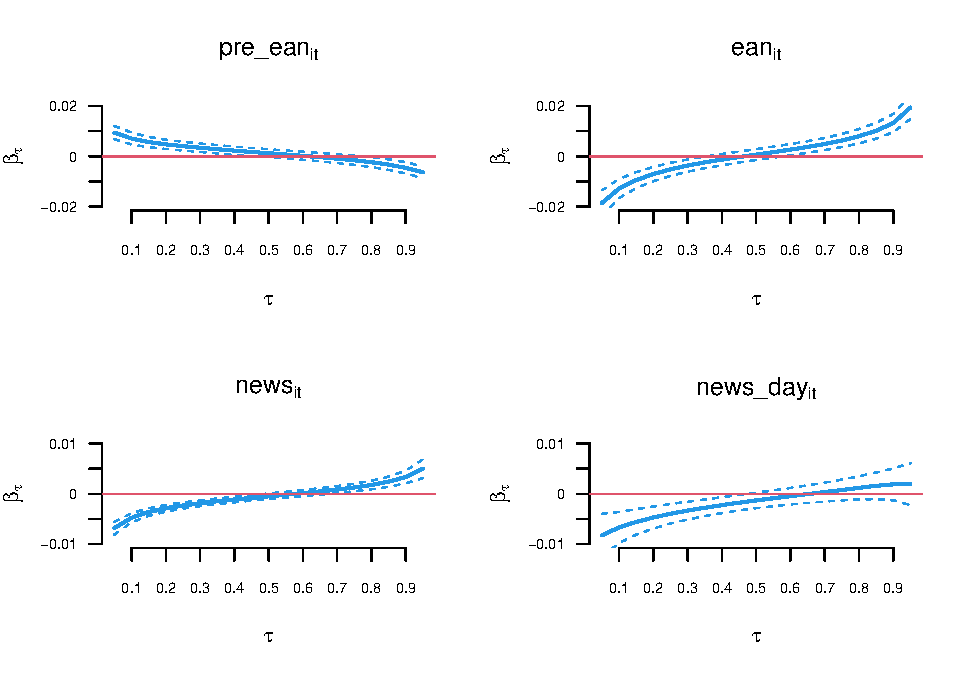
\includegraphics{sentiment_analysis_files/figure-latex/figure1-1.pdf}
\caption{\label{fig:figure1}Coefficient profiles of selected investor attention-related variables for different \(\tau\)-levels.}
\end{figure}

As reported in Table \ref{tab:table1}, many of the effects are insignificant for the conditional mean return but become significant for the conditional \(\tau\)-expectiles with \(\tau\not=0.5\). That is, higher moments of the conditional distribution are affected by the considered investment opinion proxies. Also, the explained weighted variance proportion becomes higher in the tails of the conditional return distribution.

In the Figure \ref{fig:figure1}, we plot the attention-related effects with \(95\%\)-CI in Figure \ref{fig:figure1} across the \(\tau\)-values.
Note that the effects of $ean_{i,t}$ and $news_{i,t}$ are negative for low expectiles and become positive for higher $\tau$-levels. Thus, these events tend to increase the dispersion in returns by "pushing" their expectiles apart. For the effect of $pre\_ean_{i,t}$, the opposite holds. However, the overall effect absorbs also the reversed contribution of $turn_{i,t}\cdot days\_ean_{i,t}$, such that both reduction and increase of dispersion are conceivable. The coefficient profile of $news\_day$ exhibits a significant negative impact on lower expectiles producing a potential source of negative skewness in the return distribution.


\begin{figure}[h!]
\centering
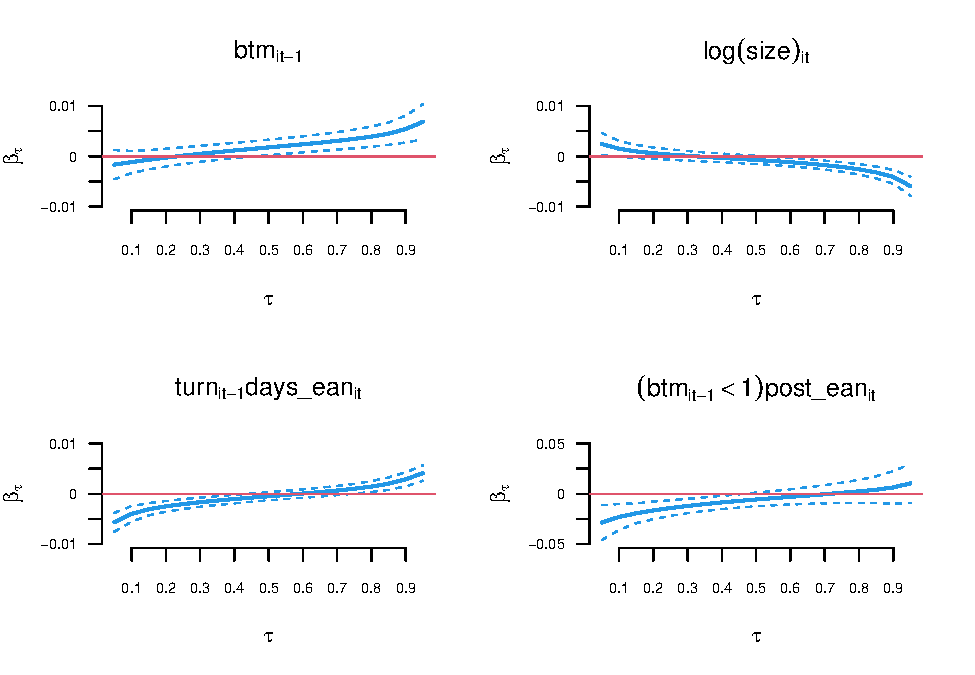
\includegraphics{sentiment_analysis_files/figure-latex/figure2-1.pdf}
\caption{\label{fig:figure2}Coefficient profiles of selected investor perception-related variables for different \(\tau\)-levels.}
\end{figure}

Figure \ref{fig:figure2} shows the effects related to investor perception with $95\%$-CI. Here, higher values of $btm$ and $turn \cdot days\_ean$ induce a higher expectile spread and, consequently, higher dispersion. The negative influence of $btm<1\cdot post\_ean$ and $log(size)$ is one-sided, directed on either low or high expectiles.

In Figure \ref{fig:figure3}, we present the effects related to investor sentiment with $95\%$-CI.
Overall, significant sentiment effects are all positive, meaning the sign of the sentiment tone determines the expected direction of the conditional return reaction. Meanwhile, $lm\_tone$ and $surp$ tend to shift the whole distribution, whereas  $hv\_tone$ show a significant impact primary on the lower expectiles.

The effect of news releases is positive for higher expectiles and is sharpened by the sign of the associated sentiment tone. Simultaneously, we observe a strongly negative effect of news arrivals for low return expectiles regardless of the news tone. That is, even news with positive content expands the gap between return expectiles and increases the dispersion of abnormal returns. This effect can be connected to the 'sidedness' of \cite{SARKAR2009} where the disproportionaly higher seller or buyer quote at news arrivals applies.

\begin{figure}[h!]
\centering
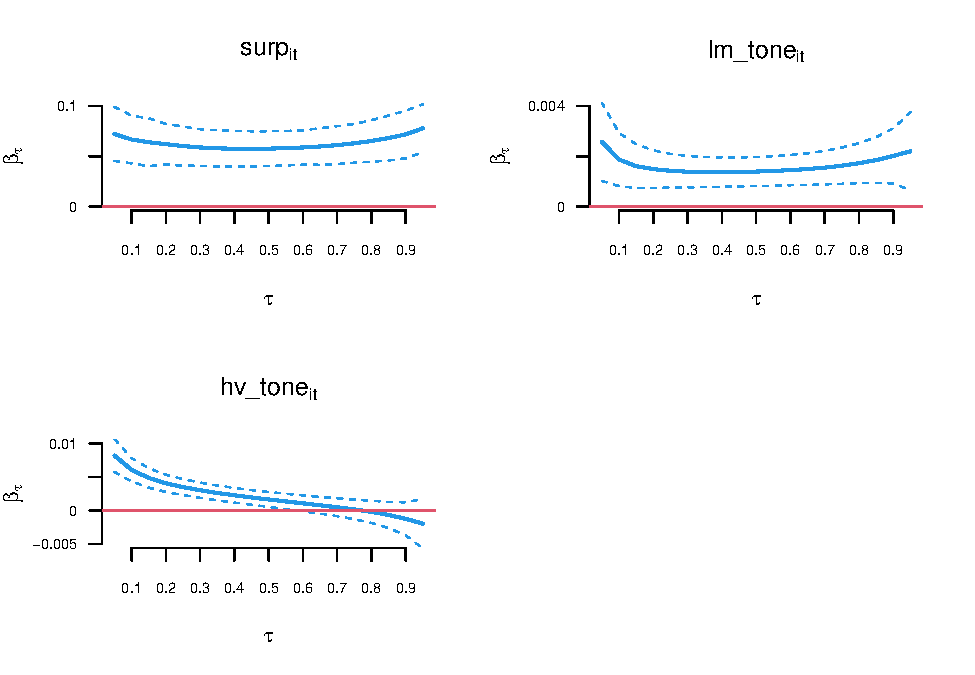
\includegraphics{sentiment_analysis_files/figure-latex/figure3-1.pdf}
\caption{\label{fig:figure3}Coefficient profiles of the investor sentiment related variables for different \(\tau\)-levels}
\end{figure}

In summary, some of the effects, such as $pre\_ean$, $ean$, $news$, $btm$, and $turn\cdot days\_ean$, impact both higher and lower expectiles with opposite effects (negative versus positive). As a result, they have a "widening" effect on the distribution as expectiles below and above the mean are pushed apart. $lm\_tone$ shifts all expectiles either to the right or to the left depending on the sign of the tone. Other considered effects are one-sided and change either the right or the left tail of the return distribution. We explore the resulting changes in shape of the conditional return distribution regarding its dispersion and skewness, as well as tail measures in the next section.


\hypertarget{quantifying-the-effects-on-the-shape-of-the-return-distribution}{%
\section{Sentiment effects on the shape of the return distribution}\label{quantifying-the-effects-on-the-shape-of-the-return-distribution}}

In this section, we quantify the effects of the considered events, such as news releases and earnings announcements, on the shape of the return distribution. To capture the latter, we use the recently proposed measures of dispertion and skewness based on expectiles (\cite{eberl2022}), as well as the connection of expectiles and expected shortfall established by \cite{Taylor2008}.

We use boostrap to check for the significance of our results. The associated confidence intervals are obtained by cross-sectional and temporal bootstrap, as defined in \cite{Kapetanios2008}, using \(1000\) bootstrap draws. To preserve possible serial dependence, we use block bootstrap with a block length of \(60\) for the time-series dimension.

\hypertarget{expectile-based-dispertion-and-skewness-measures}{%
\subsection{Expectile-based dispertion and skewness measures}\label{expectile-based-dispertion-and-skewness-measures}}

The estimated conditional expectile model coefficients facilitate a comparison of the resulting distributional effects via expectile-based shape measures. One useful concept - \emph{interexpectile difference} (or range) - was introduced in the financial context by \cite{bellini2018} to measure the variability of a risk-neutral distribution. Their interexpectile difference for a random variable \(X\) with a finite expectation \(\mathbb E(X)\) is defined for \(\tau\in(0,0.5)\) as:

\[\Delta_\tau = e_{1-\tau}(X) - e_\tau(X).\]


The authors show that the proposed measure is consistent with the convex order. Recently, \cite{eberl2022} demonstrated that the empirical interexpectile range is more efficient than the classical standard deviation for skewed and long-tailed distributions. Moreover, a class of expectile-based measures of skewness was proposed in \cite{eberl2022sk}. Here we use their \(s_{2\tau}\) (denoted further as \(s_\tau\)), defined as:

\[s_{\tau} = \frac 1{1-2\tau}\cdot\frac{e_{1-\tau}(X) + e_\tau(X) - 2\mathbb E(X)}{e_{1-\tau}(X) - e_\tau(X)}\]

for \(\tau\in(0,0.5).\) This skewness measure is normalized to \((-1,1)\) and has the property \(s_2(\tau)\geq 0\) (\(s_2(\tau)\leq 0\)) whenever \(\tau\in(0,0.5)\) and the distribution is right-skewed (left-skewed).

We take \(\tau=0.1\) for our analysis, which was also used in \cite{eberl2022sk}, and consider the straight forward adjustment for our conditional expectile regression setup of the model in \eqref{eq:mod0}. In our case, the conditional interexpectile range for $\tau=0.1$ becomes :
\[\Delta_{0.1,i,t} = e_{0.9,t}(r_{i,t}) -  e_{0.1,t}(r_{i,t}) = x_{i,t}^\top (\beta_{0.9} - \beta_{0.1}) + z_i^\top(\gamma_{0.9} - \gamma_{0.1}),\]
where $x_{i,t}$ is a vector of the time-varying firm characteristics from (\ref{eq:mod0}), and $z_i$ is a vector of firm characteristics that do not change over time. Similarly, conditional expectile-based skewness measure $\hat s_{\tau,i,t}$ for $\tau=0.1$ is:
\begin{align*}s_{0.1,i,t} &= \frac 1{1-2\cdot0.1}\cdot\frac{e_{0.9,t}(r_{i,t}) + e_{0.1,t}(r_{i,t}) - 2e_{0.5,t}(r_{i,t})}{\Delta_{0.1,i,t}}\\
&=1.25\cdot\frac{x_{i,t}^\top (\beta_{0.9} + \beta_{0.1} - 2\beta_{0.5}) + z_i^\top(\gamma_{0.9} + \gamma_{0.1} - 2\gamma_{0.5})}{x_{i,t}^\top (\beta_{0.9} - \beta_{0.1}) + z_i^\top(\gamma_{0.9} - \gamma_{0.1})}.
\end{align*}

The plugin the estimator for the conditional interexpectile range becomes:
\[\hat\Delta_{0.1,i,t} = x_{i,t}^\top (\hat\beta_{0.9} - \hat\beta_{0.1}) + z_i^\top(\hat\gamma_{0.9} - \hat\gamma_{0.1}),\]
and the one for conditional expectile-based skewness $\hat s_{\tau,i,t}$ reads:
\begin{align*}\hat s_{0.1,i,t} &= 1.25\cdot\frac{x_{i,t}^\top (\hat\beta_{0.9} + \hat\beta_{0.1} - 2\hat\beta_{0.5}) + z_i^\top(\hat\gamma_{0.9} + \hat\gamma_{0.1} - 2\hat\gamma_{0.5})}{x_{i,t}^\top (\hat\beta_{0.9} - \hat\beta_{0.1}) + z_i^\top(\hat\gamma_{0.9} - \hat\gamma_{0.1})}.
\end{align*}

To assess the average effects of sentiment events, such as news arrivals or earnings announcements, on the considerred interexpectile range and skewness for each firm $i$ and each time $t$,  we first compute \(\hat\Delta_{0.1,i,t}\) and $\hat s_{0.1,i,t}$. Then, we average the resulting values over the firms and time indices with a particular sentiment event. The polarity (positive or negative) of a sentiment event is assessed via the sign of the earnings suprises in case of $ean$ and $post\_ean$, and via the dictionary-based textual sentiment (the average of $lm\_tone$ and $hv\_tone$) for $pre\_ean$ and $news$. The resulting means are denoted as \(\overline\Delta_{0.1}^{no~event}\), \(\overline\Delta_{0.1}^{event}\), and $\overline s_{0.1}^{event}$. The associated significant changes in the interexpectile ranges for the sentiment events, \(\overline\Delta^{event}_{0.1}-\overline\Delta^{no~event}_{0.1}\), as well as the increase factors, \(\overline\Delta^{event}_{0.1}/\overline\Delta^{no~event}_{0.1}\), are provided in Table \ref{tab:tabdelt1}. As already mensioned, significance is obtained via cross-sectional and temporal bootstrap.

\begin{table}[ht]
\centering
\caption{\label{tab:tabdelt1}Mean interexpectile ranges $\overline\Delta^{event}_{0.1}$ and mean expectile-based skewness $\overline s^{event}_{0.1}$ on event days. The increases in dispersion compared to the case of no event ($\overline\Delta^{event}_{0.1}-\overline\Delta^{noevent}_{0.1}$) are given in brackets.  Symbols '***','**','*' indicate significance on 0.1\%, 1\%, 5\% level respectively by bootstrap confidence intervalls.}
\begin{tabular}{llll}
  \hline
 event & $\overline\Delta_{0.1}^{event} (\overline\Delta_{0.1}^{event} - \overline\Delta_{0.1}^{noevent} )$ & $\overline\Delta_{0.1}^{event} /\overline\Delta_{0.1}^{noevent} $ & $\overline s_{0.1}^{event}$\\
  \hline
noevent & 0.021~~(-) & 1.00 & ~0.0044 \\
pre\_ean\_positive	& 0.024~~({\bf0.0025}*) & 1.12 & -0.0079\\
pre\_ean\_negative	& 0.0308~({\bf0.0093}***) & 1.43 & -0.0469\\
 %pre\_ean & 0.0253 (0.0037***) & 1.17 & -0.0154 \\
 news\_positive & 0.0253~({\bf0.0038}***) & 1.18 & ~{\bf0.0244}*\\
 news\_negative & 0.0273~({\bf0.0059}***) & 1.3 & {\bf-0.0395}*\\
 ean\_positive & 0.0589~({\bf0.0374}***) & 2.74& -0.0069\\
  ean\_negative & 0.0648~({\bf0.0433}***) & 3.02 & -0.0398\\
  post\_ean\_positive & 0.0803~({\bf0.0588}***) & 3.74& ~0.0012\\
  post\_ean\_negative & 0.0851~({\bf0.0636}***) & 3.96& ~0.0061\\
   \hline
\end{tabular}
\end{table}

We observe a substantial increase in dispersion on days around earnings announcements\footnote{A significant increase of the dispersion on the days before earnings announcements shows up only for negative sentiment and results from the interplay of the effects of sentiment variables, \(pre\_ean\) and \(turn*days\_ean\). }.  This effect possibly traces back, according to \cite{BERKMAN2009}, to opinion differences and opinion alignment after earnings announcements. Our findings confirm, therefore, the results of previous studies detecting increase in volatility on such event days. Also, the asymmetric effect on dispertion resulting in higher increase of the interexpectile ranges in cases where the sentiment is negative, aligns with recently provided evidence on attention-based trading in \cite{barber2022}.  The effect of positive or negative news  arrivals on the changes in interexpectile range is much more subtle. News releases enhance the increase in dispersion of over 20\% on average.

In addition, the resulting per-event average expectile-based skewness, $\overline s_{0.1}^{event}$, is also presented in Table  \ref{tab:tabdelt1}. It reveals that news releases induce significant positive and negative skewness of the return distribution, when textual news polarity is positive or negative, respectively, which generalizes the previous findings of \cite{ekholm2007} for the case of negative news releases.


\hypertarget{impact-of-investor-opinion-on-the-conditional-expected-shortfall-of-the-returns}{%
\section{The impact of the investor opinion channels on the conditional expected shortfall}\label{impact-of-investor-opinion-on-the-conditional-expected-shortfall-of-the-returns}}

A frequently used risk measure is the \(\alpha\)-expected shortfall, denoted as \(ES_{\alpha}\). It is connected to the quantile \(q_\alpha\) of the target distribution. For the lower tail of the latter, this risk measure is defined as \(ES_\alpha = \mathbb E(Y|Y<q_\alpha)\).

\cite{JONES1994} shows that there is a one-to-one correspondence between quantiles and expectiles of a continuous distribution. Based on that, \cite{Taylor2008} proposes to use expectiles to estimate $ES_{\alpha}$ with $\alpha\leq 0.5$ via:


\begin{align}
{ES}_{\alpha} &= \left(1+\frac{\tau}{(1-2\tau)\alpha}\right)e_{\tau} - \frac{\tau}{(1-2\tau)\alpha}e_{0.5},
\end{align}

where \(\alpha\in(0,0.5]\) denotes the quantile level, \(\tau\in(0,1)\) is the associated expectile level, and \(e_{\tau}\) is the respective expectile. As \cite{Taylor2008} mentions, the same relation holds for the conditional expected shortfall with respect to the conditional expectile.

\cite{yao1996} show the existence of a bijective function \(\tau:(0,1)\rightarrow (0,1)\) which connects the quantile level \(\alpha\) to the expectile level \(\tau\) such that \(q_\alpha = e_{\tau(\alpha)}\).

Thus, if the relation \(\hat\tau(\alpha)\) or its estimate \(\hat \tau(\alpha)\) is available, a plug-in estimator for the expected conditional shortfall based on the estimated conditional expectile analog to the autoregressive version in \cite{Taylor2008} can be obtained:

\begin{align}
\widehat{ES}_{\alpha}(r_{i,t}|x_{i,t},z_i) &= \left(1+\frac{\hat\tau(\alpha)}{\big(1-2\hat\tau(\alpha)\big)\alpha}\right)\hat e_{\hat\tau(\alpha)}(r_{i,t}|x_{i,t},z_i) - \frac{\hat\tau(\alpha)}{\big(1-2\hat\tau(\alpha)\big)\alpha}\hat e_{0.5}(r_{i,t}|x_{i,t},z_i)\nonumber\\
&=\tilde \beta_{0,\alpha} + \tilde\beta_{\alpha}^\top \cdot x_{i,t} + \tilde\gamma_\alpha^\top\cdot z_i,\label{eq:es}
\end{align}

with
\begin{equation}\tilde\beta_\alpha = \hat \beta_{\hat\tau(\alpha)} - \frac{\hat\tau(\alpha)}{\big(1-2\hat\tau(\alpha)\big)\alpha}\cdot \left(\hat\beta_{0.5} -\hat \beta_{\hat\tau(\alpha)}\right)\label{eq:tbeta}
\end{equation}

and \(\tilde\beta_0\) and \(\tilde\gamma\) are defined analogous.

To obtain the actual estimates, we first estimate the conditional expectile model as in \eqref{eq:mod0} for a fine grid of \(\tau = 0.001, 0.0025, 0.005,0.01,0.02,\ldots, 0.1\). Following \cite{Taylor2008}, we construct an empirical cumulative distribution function by counting the observations below the estimated expectile profile for each of the \(\tau\)-levels, such that for each \(\tau\) we have the corresponding quantile index \(\alpha\). We then interpolate linearly between the resulting points to obtain \(\hat\tau(\alpha)\) particular for \(\alpha\in\{0.01,0.05,0.1\}\). The estimated correspondence is plotted in the left plot of Figure \ref{fig:figure4}.

For instance, in our model specification, the lower quantile levels \(\alpha\in\{0.01,0.05,0.1\}\) correspond to the expectile levels \(\tau\in\{0.0027,0.0214,0.0533\}\) respectively, see also Figure \ref{fig:figure4}.

\begin{figure}\label{fig:figure4}
\centering
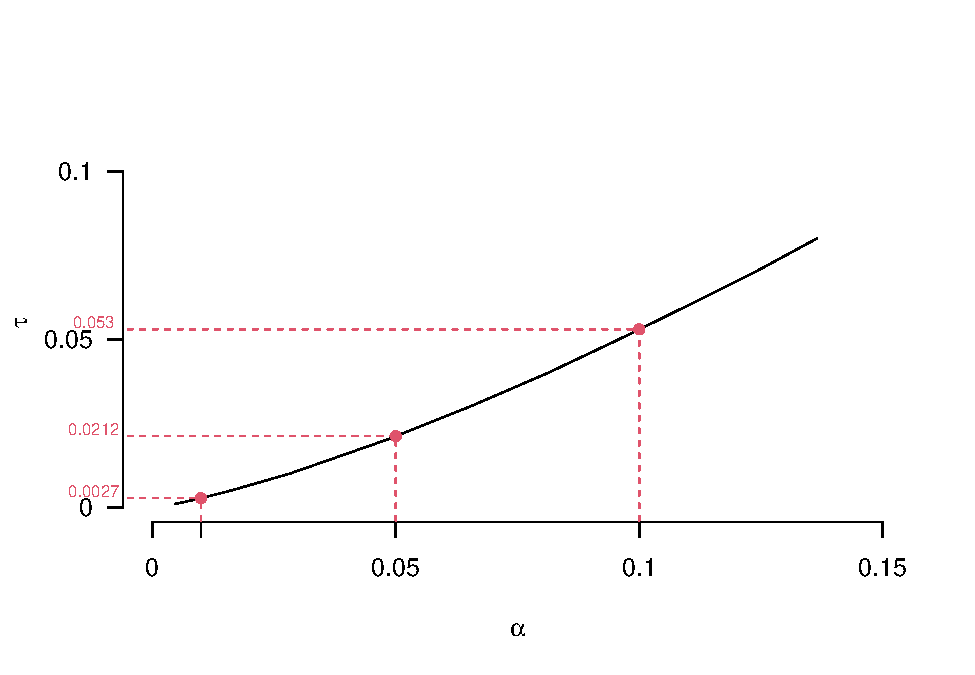
\includegraphics[width=0.45\textwidth]{sentiment_analysis_files/figure-latex/figure4-1}
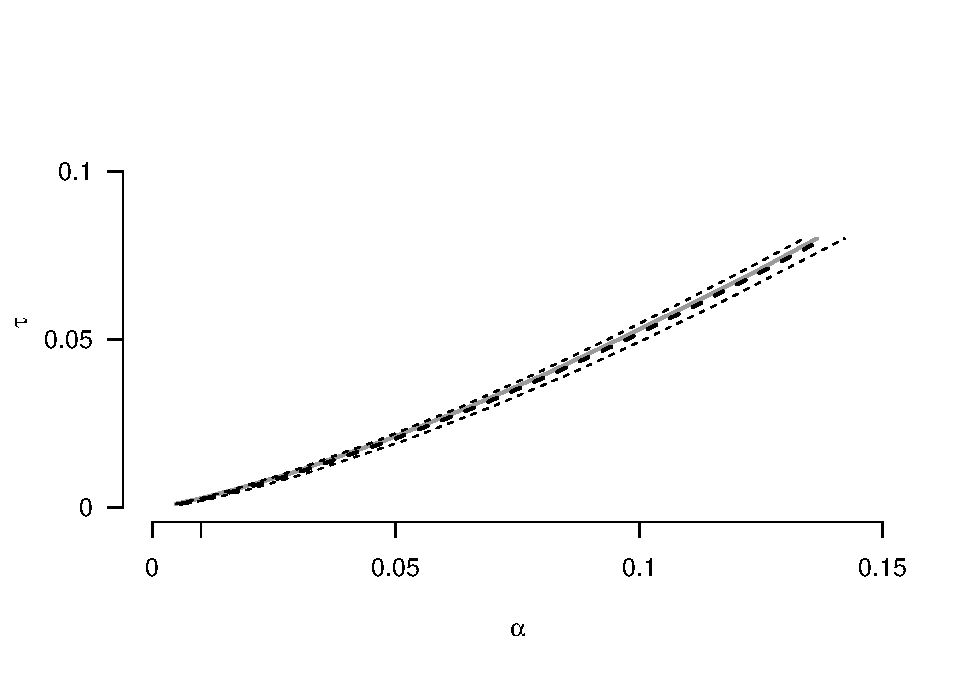
\includegraphics[width=0.45\textwidth]{sentiment_analysis_files/figure-latex/figure5-1}
\caption{The estimated relation between the expectile level \(\tau\) and the quantile level \(\alpha\) for the NASDAQ return distribution. The left plot shows  estimated $\tau(\alpha)$ with expectile levels shown for quantile levels \(\alpha\in\{0.01,0.05,0.1\}\). The right plot shows estimated $\tau(\alpha)$ using the original NASDAQ return data (solid line) with boostrap based mean and $95\%$ confidence intervals (dashed lines).}\vspace{-0.5cm}
\end{figure}


For the target \(\alpha\in\{0.01,0.05,0.1\}\), we compute the resulting coefficients \(\tilde\beta_\alpha\) representing the investor opinion effects on the conditional expected shortfall.

The bootstrapping is carried out as follows: For each bootstrap draw \(b=1,\ldots, B\), we first estimate the ER model for a fine grid of \(\tau\)-values in the left tail \(0.001,0.0025,0.005,0.01,0.02,\ldots,0.1\). Then, using the fitted conditional expectiles, we estimate the correspondence \(\hat\tau^{(b)}(\alpha)\) by assigning to each \(\tau\)-value the proportion of observations \(\alpha\) in the bootstrap sample lying below the expectile profile \(\{e_{\tau}(r^{(b)}_{it})\}_{i=1,t=1}^{N,T}\). By interpolating linearly between the points, we determine the needed \(\tau\)-levels for the target \(\alpha\)-levels of \(0.01,0.05,0.1\). The estimated \(\hat\tau(\alpha)\) with \(95\%\) bootstrap confidence intervals is presented in the right plot of Figure \ref{fig:figure4}.

Finally, we compute \(\tilde\beta^{(b)}_\alpha\) for each bootstrap sample as specified in \eqref{eq:tbeta}, i.e.:
$\tilde\beta^{(b)}_\alpha = \hat \beta^{(b)}_{\hat\tau^{(b)}(\alpha)} - \frac{\hat\tau^{(b)}(\alpha)}{\big(1-2\hat\tau^{(b)}(\alpha)\big)\alpha}\cdot \left(\hat\beta_{0.5} -\hat \beta_{\hat\tau^{(b)}(\alpha)}\right).$
Based on the resulting bootstrap distribution of \(\left\{\tilde\beta^{(b)}_\alpha\right\}_{b=1}^B\), we then construct the confidence intervals.
%The same procedure is used to obtain the bootstrap confidence intervals for $\tilde\gamma_\alpha$.

\begin{table}[h!]

\caption{\label{tab:unnamed-chunk-22}The estimated coefficients $\tilde\beta_\alpha$ (computed as bootstrap means) measuring the effects of investor opinion on the expected shortfall. '***', '**', and '*' indicate significance of 0.001, 0.01, and 0.05 respectively obtained based on boostrap confidence intervalls.}
\centering
\begin{tabular}[t]{l|l|l|l}
\hline
  & $ES_{0.01}$ & $ES_{0.05}$ & $ES_{0.1}$\\
\hline
Constant & -0.3036 & -0.1681 & -0.125\\
\hline
$pre\_ean_{i,t}$& ~0.0227** & ~0.0172*** & ~0.0137***\\
\hline
$ean_{i,t}$  & -0.0525*** & -0.0374*** & -0.0291***\\
\hline
$post\_ean_{i,t}$ & -0.0093 & -0.0125 & -0.0104\\
\hline
$news\_{i,t}$ & -0.0242*** & -0.0139*** & -0.0102***\\
\hline
$news\_sector_{i,t}$  & ~0.0019 & ~0.0016 & ~0.0018\\
\hline
$news\_day_{i,t}$ & -0.0126 & -0.014 & -0.0126*\\
\hline
$\log(size_{i,t})$ & ~0.0092 & ~0.0047 & ~0.0034\\
\hline
$btm_{i,t-1}$ & -0.0015 & -0.0027 & -0.0029\\
\hline
$turn_{i,t-1}\cdot days\_ean_{i,t}$ & -0.0139* & -0.011*** & -0.0085***\\
\hline
$(btm_{i,t-1}\leq 1)\cdot post\_ean_{i,t}$ & -0.0711** & -0.0498* & -0.0403\\
\hline
$supr_{i,t}$& ~0.0831 & ~0.1028 & ~0.093*\\
\hline
$lm\_tone_{i,t}$& ~0.0112 & ~0.0051 & ~0.0031\\
\hline
$hv\_tone_{i,t}$& ~0.0221 & ~0.0158** & ~0.0119***\\
\hline
\end{tabular}
\end{table}

For \(\alpha = 0.01,0.05\) and \(0.1\), we confirm significant effects of \(pre\_ean\),  \(ean\), \(news\), and turnover around earnings announcements \(turn\cdot days\_ean\); the post earnings announcements  \((btm\leq 1)\cdot post\_ean\) shows an effect for \(\alpha=0.01, 0.05\). $ES_{0.1}$ seems to be impacted also by $news\_day_{i,t}$ and $supr_{i,t}$. The effect of \(lm\_tone\) is  insignificant. However, for \(hv\_tone\), we find a significant effect for \(\alpha=0.05\) and \(0.1\).

%As in the case of the conditional expectile model, earnings announcements and share turnover around earnings announcements exhibit significant negative effects on the conditional expected shortfall. Also, the combination of a positive effect of \(pre\_ean\) and a negative effect of \(ean\) and \(news\)) persists in the conditional expected shortfall model, making it relevant risk management.

Based on our bootstrap procedure, we confirm significant effects of \(pre\_ean\), \(ean\), and \(news\) on \(ES_\alpha\) with \(\alpha=0.01,0.05,0.1\). Besides that, turnover around earnings announcements \(turn\cdot days\_ean\) and text sentiment \(hv\_tone\) show significant impacts on \(ES_{0.05}\) and \(ES_{0.1}\).

As in the case of the conditional expectile model, earnings announcements and share turnover around earnings announcements exhibit significant negative effects on the conditional expected shortfall. Significant effects of \(pre\_ean\) , \(ean\) and $news$ persist in the conditional expected shortfall consideration. Also, the overall singificant asymmetric effect of news releases with positive and negative sentiment is confirmed for the case of $ES_{0.05}$ and  $ES_{0.1}$,  making it relevant for risk management.

\hypertarget{conclusion}{%
\section{Conclusion}\label{conclusion}}

We conducted an analysis of the distributional effects of  investor opinion on asset prices using a panel of abnormal NASDAQ returns covering the time period from April 2015 to August 2019. Our approach is based on the information flow structure proposed  by \cite{Su2021}, where investor is characterized by channels such as investor attention, perception, and sentiment. Proxies for each of these channels, drawn from previous studies, served as covariates in an expectile regression model introduced  by \cite{Newey1987}. We utilized abnormal return as a response variable to evaluate distributional effects beyond conditional mean regression, without making assumptions about the response distribution.

The majority of estimated effects are dependent on the expectile level, denoted as the ``extremeness'' \(\tau\), in a nonlinear manner. The associated estimates change sign when moving from the left to the right tail, or vice versa, of the conditional response distribution. A detailed analysis of attention-grabbing events, such as news releases and days around earnings announcements, with positive and negative sentiment reveals a significant asymmetric increase in dispersion, measured by the interexpectile range, occurring on event days. Particularly noteworthy is the asymmetric skewness effect of news, measured through expectile skewness, where positive/negative news induces significant left/right skewness of the distribution. One plausible explanation for the change in skewness could be the ``market sideness'' of \cite{SARKAR2009}. Moreover, analogous significant effects are found in the conditional expected shortfall model, which we obtain by incorporating our conditional expectile formulation into the expected-shortfall-expectile relation derived by \cite{Taylor2008}. These findings have important implications for the risk management assessment of investor opinion formation channels.

A potential direction for future research could involve extending investor sentiment to topic-based representations and assessing the effect of different news topics on the conditional distribution and conditional expected shortfall of stock returns.



%%%%%%%%%%%%%%%%%%%%%%%%%%%%%%%%%%%%%%%
\bibliographystyle{jasa}
\bibliography{references}

%%%%%%%%%%%%%%%%%%%%%%%%%%%%%%%%%

\newpage
\hypertarget{appendix}{
\section*{Appendix}\label{appendix}}

\hypertarget{list-of-the-firm-tickers-in-the-dataset}{%
\subsection*{List of the firm tickers in the dataset}\label{list-of-the-firm-tickers-in-the-dataset}}

`AAPL', `AMZN', `TSLA', `FB', `BA', `NFLX', `DIS', `EFX', `BAC', `INTC', `F', `GE', `GM',
`MSFT', `SBUX', `AIR', `AAL', `IBM', `JPM', `CMG', `WFC', `C', 
`TWTR', 
`WMT', `MCD', `AMD', `NVDA', `JNJ', `GS',
`BABA', `CAT', `MU', `CSCO', `XOM', `CVX', `BP', `GOOGL', `GPRO', `COST', `HD', `NKE', `KO',
`AXP', `TGT', 
`ATVI', 
`CMCSA', `DAL', `LMT', `T', `ABBV', `PFE', `GILD', `ADBE', `CRM', `VZ', `AVGO', `BX',
`LULU', `BLK', `UNH', `KMI', `BBY', `PG', `AGI', `AMAT', `MRK', `M', `BIDU', `QCOM', `FDX', `AMGN',
`BMY', `ORCL', 
%`BHP',
 `MA', `KR', `MO', `GME', `PM', `CHK', `MMM', 
%`BBBY', 
`COP', `IRBT', `MS',
`FCX', `HAL', `HPQ', `UAL',`JWN', `CVS', `V', `EA', `STZ', `GLW', `ADP', `AZN', `EBAY', `ACN', `PEP'.

\hypertarget{news-article-data}{%
\subsection*{News article data}\label{news-article-data}}

%In total, we have 30,424 news articles, and the average word count of the final news article sample is 1,114.
\vspace{-0.5cm}
\begin{table}[ht!]

\caption{\label{tab:table00}Description of the final textual corpus}
\centering
\begin{tabular}[t]{l|l|l}
\hline
Year & News Articles (merged) & Average Word Count\\
\hline
2015 & 4,395 & 823\\
\hline
2016 & 5,391 & 840\\
\hline
2017 & 5,738 & 923\\
\hline
2018 & 8,465 & 1,352\\
\hline
2019 & 6,435 & 1,401\\
\hline
All years & 30,424 & 1,114\\
\hline
\end{tabular}
\end{table}


\hypertarget{empirical-data-summary}{%
\subsection*{Empirical data summary}\label{empirical-data-summary}}

We provide a standard summary of data for each variable in Table \ref{tab:table01} and Table \ref{tab:table02}, a time period and sector wise expectile summaries of the return distributions in Table \ref{tab:table03} and Table \ref{tab:table04}, and per-expectile summary of explanatory variables to give the reader an overview of the data structure in Table \ref{tab:table05}.

\begin{table}[h!]

\caption{\label{tab:table01}Summary statistics for the variables: daily firm excess returns $r$, the logarithm of firm size $\log(size)$, firm btm ratio $btm$, and shares turnover $turn$.}
\centering
\begin{tabular}[t]{l|l|l|l|l}
\hline
  & $r_{\cdot,\cdot}$ & $\log(size_{\cdot,\cdot})$ & $btm_{\cdot,\cdot}$ & $turn_{\cdot,\cdot}$\\
\hline
%min & -0.36198 & 19.60939 & 0.00000 & 0.26464\\
% max & 0.52106 & 27.72950 & 4.48289 & 17.60180\\
  mean & 0.0001 & 24.8414& 0.3851& 1.8233\\
\hline
  sd & 0.0170 & ~~1.4000 & 0.4316& 1.9147\\
\hline
  skewness & 0.3375 & ~-0.9917 & 2.9686 & 3.1539\\
\hline
\end{tabular}
\end{table}

\begin{table}[h!]

\caption{\label{tab:table02}Summary statistics for the variables: earning surprise $supr$ only for the days of earnings announecements, news sentiment based on LM dictionary denoted as $lm\_tone$ and on HV dictionary denoted as $hv\_tone$ for the days of news releases.}
\centering
\begin{tabular}[t]{l|r|r|r|r}
\hline
  & $supr$ &$eps$ &$lm\_tone$ & $hv\_tone$ \\
%\hline
%min & -11.87825 & -2.15000 & -1.00000 & -1.00000\\
%\hline
%  max & 22.92849 & 7.52000 & 1.00000 & 1.00000\\
\hline
 mean & 2.4436 & 1.3360 & -0.0461 & 0.3845\\
\hline
sd & 7.8944& 1.5414& 0.4581 & 0.2135\\
\hline
 skewness & 3.0959 & 3.0267& 0.0634 & -0.5590\\
\hline
\end{tabular}
\end{table}



In Table \ref{tab:table03} empirical return expectiles \(\hat e_{\tau}\) for \(\tau = 0.05,0.25,0.5,0.75,\) and \(0.95\) and different sub periods of the considered time span are reported. We observe that the tail indices remain approximately the same over time. In Table \ref{tab:table04} we report the empirical return expectiles \(\hat e_{\tau}\) for \(\tau = 0.05,0.25,0.5,0.75,\) and \(0.95\) sector wise.


\begin{table}[h!]

\caption{\label{tab:table03}Empirical expectiles for the excess returns for the whole time span 2015-2019, for the first sub period 2015-2016 and for the second sub period 2017-2019.}
\centering
\begin{tabular}[t]{l|l|l|l|l|l}
\hline
  & $\hat e_{0.05}$ & $\hat e_{0.25}$ & $\hat e_{0.5}$ & $\hat e_{0.75}$ & $\hat e_{0.95}$\\
\hline
2015-2019 & -0.0189 & -0.0058 & 0.0001 & 0.0060 & 0.0192\\
\hline
2015-2016 & -0.0194 & -0.0058 & 0.0002 & 0.0062 & 0.0206\\
\hline
2017-2019 & -0.0186 & -0.0058 & 0.0000 & 0.0059 & 0.0184\\
\hline
\end{tabular}
\end{table}

\begin{table}[h!]

\caption{\label{tab:table04}Empirical expectiles for the excess returns for the whole time span 2015-2019 for each of the ten sectors}
\centering
\begin{tabular}[t]{l|l|l|l|l|l}
\hline
 Sector & $\hat e_{0.05}$ & $\hat e_{0.25}$ & $\hat e_{0.5}$ & $\hat e_{0.75}$ & $\hat e_{0.95}$\\
\hline
Basic Materials & -0.0393 & -0.0136 & 0.0001 & 0.0143 & 0.0433\\
\hline
Consumer Discretionary & -0.0197 & -0.0061 & 0.0000 & 0.0060 & 0.0191\\
\hline
Consumer Staples & -0.0158 & -0.0050 & 0.0000 & 0.0050 & 0.0151\\
\hline
Energy & -0.0245 & -0.0079 & -0.0005 & 0.0072 & 0.0255\\
\hline
Finance & -0.0122 & -0.0041 & 0.0001 & 0.0044 & 0.0130\\
\hline
Health Care & -0.0143 & -0.0048 & -0.0001 & 0.0046 & 0.0138\\
\hline
Industrials & -0.0139 & -0.0044 & 0.0003 & 0.0050 & 0.0146\\
\hline
Technology & -0.0196 & -0.0057 & 0.0005 & 0.0068 & 0.0215\\
\hline
Telecommunications & -0.0115 & -0.0038 & 0.0002 & 0.0041 & 0.0119\\
\hline
Utilities & -0.0193 & -0.0069 & -0.0007 & 0.0057 & 0.0190\\
\hline
\end{tabular}
\end{table}

Here we observe substantial variation of empirical expectiles between sectors. Based on this observation, we include sector and firm dummies to account for the posible individual variability and the variability across sectors.

In the following Table \ref{tab:table05} per-expectile distributional summary is displayed. The summary statistics for the explanatory variables is conditioned on excess returns belonging to a specific empirical expectile interval: \([\min(r), \hat e_{0.05})\), \([\hat e_{0.05}, \hat e_{0.25} )\), \([\hat e_{0.25}, \hat e_{0.5})\), \([\hat e_{0.5}, \hat e_{0.75})\), \([\hat e_{0.75}, \hat e_{0.95})\), and \([\hat e_{0.95}, \max(r)]\). We report the mean and the standard deviation in parenthesis for the variables.


\begin{table}[h!]

\caption{\label{tab:table05}Per-expectile means (standard deviations) of the variables shares turnover $turn$, logarithm of size $\log(size)$, btm ratios $btm$, indicator of news arrivals $news$, and indicator of earnings announcements $ean$.}
\centering
\begin{tabular}[t]{l|l|l|l|l|l|l}
\hline
  & $turn$ & $\log(size)$ & $btm$ & $news$ & $ean$&$eps$\\
\hline
{\scriptsize{$r\leq \hat e_{ 0.05 }$}} & 3.14 (2.87) & 23.97 (1.64) & 0.43 (0.46) & 0.31 (0.46) & 0.048 (0.21) & 1.22 (1.15)\\
\hline
{\scriptsize{$\hat e_{ 0.05 }\leq r\leq \hat e_{ 0.25 }$}} & 1.86 (1.87) & 24.79 (1.38) & 0.40 (0.44) & 0.25 (0.43) & 0.011 (0.11) & 1.35 (1.26)\\
\hline
{\scriptsize{$\hat e_{ 0.25}\leq r\leq \hat e_{ 0.5 }$}} & 1.42 (1.36) & 25.07 (1.24) & 0.37 (0.42) & 0.23 (0.42) & 0.009 (0.09) & 1.61 (1.69)\\
\hline
{\scriptsize{$\hat e_{ 0.5 }\leq r\leq \hat e_{ 0.75 }$ }}& 1.44 (1.44) & 25.07 (1.24) & 0.36 (0.40) & 0.23 (0.42) & 0.009 (0.09) & 1.42 (1.64)\\
\hline
{\scriptsize{$\hat e_{ 0.75 }\leq r\leq \hat e_{ 0.95 }$}} & 1.82 (1.84) & 24.81 (1.38) & 0.38 (0.43) & 0.25 (0.44) & 0.015 (0.12) & 1.57 (1.73)\\
\hline
{\scriptsize{$r\geq \hat e_{ 0.95 }$}} & 3.06 (2.77) & 24.03 (1.62) & 0.44 (0.48) & 0.31 (0.46) & 0.052 (0.22) & 1.43 (1.52)\\
\hline
\end{tabular}
\end{table}

Interestingly, the extreme return states \(r\leq \hat e_{0.05}\) and \(r\geq \hat e_{0.95}\) are associated with substantially higher mean turnover and earnings announcements arrivals, slightly lower mean size and somewhat higher mean btm ratios and news arrivals rate.


Based on the data description above, one expects possibly different effects of the considered covariates on the location, scale and shape of the conditional return distribution. As in the summaries above, it is possible to represent the conditional return distribution through its conditional expectiles. A consistent estimator of the heterogeneous effects over the return distribution can be obtained by expectile regression.
\end{document}
